% This file was created with tikzplotlib v0.10.1.
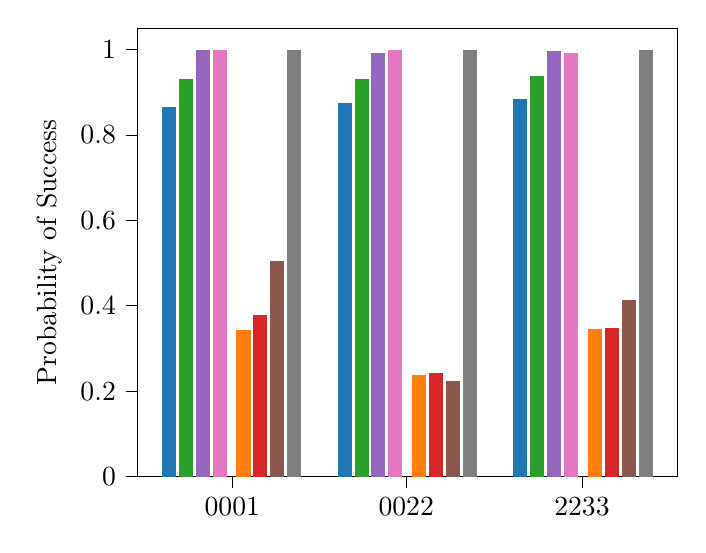
\begin{tikzpicture}

\definecolor{crimson2143940}{RGB}{214,39,40}
\definecolor{darkgray176}{RGB}{176,176,176}
\definecolor{darkorange25512714}{RGB}{255,127,14}
\definecolor{forestgreen4416044}{RGB}{44,160,44}
\definecolor{gray127}{RGB}{127,127,127}
\definecolor{mediumpurple148103189}{RGB}{148,103,189}
\definecolor{orchid227119194}{RGB}{227,119,194}
\definecolor{sienna1408675}{RGB}{140,86,75}
\definecolor{steelblue31119180}{RGB}{31,119,180}

\begin{axis}[
tick align=outside,
tick pos=left,
x grid style={darkgray176},
xmin=-0.1796, xmax=2.8916,
xtick style={color=black},
xtick={0.36,1.35,2.35},
xticklabels={0001,0022,2233},
y grid style={darkgray176},
ylabel={Probability of Success},
ymin=0, ymax=1.05,
ytick style={color=black}
]
\draw[draw=none,fill=steelblue31119180] (axis cs:-0.04,0) rectangle (axis cs:0.04,0.866);
\draw[draw=none,fill=steelblue31119180] (axis cs:0.96,0) rectangle (axis cs:1.04,0.876);
\draw[draw=none,fill=steelblue31119180] (axis cs:1.96,0) rectangle (axis cs:2.04,0.884);
\draw[draw=none,fill=darkorange25512714] (axis cs:0.384,0) rectangle (axis cs:0.464,0.344);
\draw[draw=none,fill=darkorange25512714] (axis cs:1.384,0) rectangle (axis cs:1.464,0.238);
\draw[draw=none,fill=darkorange25512714] (axis cs:2.384,0) rectangle (axis cs:2.464,0.345);
\draw[draw=none,fill=forestgreen4416044] (axis cs:0.056,0) rectangle (axis cs:0.136,0.93);
\draw[draw=none,fill=forestgreen4416044] (axis cs:1.056,0) rectangle (axis cs:1.136,0.932);
\draw[draw=none,fill=forestgreen4416044] (axis cs:2.056,0) rectangle (axis cs:2.136,0.937);
\draw[draw=none,fill=crimson2143940] (axis cs:0.48,0) rectangle (axis cs:0.56,0.378);
\draw[draw=none,fill=crimson2143940] (axis cs:1.48,0) rectangle (axis cs:1.56,0.242);
\draw[draw=none,fill=crimson2143940] (axis cs:2.48,0) rectangle (axis cs:2.56,0.348);
\draw[draw=none,fill=mediumpurple148103189] (axis cs:0.152,0) rectangle (axis cs:0.232,1);
\draw[draw=none,fill=mediumpurple148103189] (axis cs:1.152,0) rectangle (axis cs:1.232,0.991);
\draw[draw=none,fill=mediumpurple148103189] (axis cs:2.152,0) rectangle (axis cs:2.232,0.996);
\draw[draw=none,fill=sienna1408675] (axis cs:0.576,0) rectangle (axis cs:0.656,0.505);
\draw[draw=none,fill=sienna1408675] (axis cs:1.576,0) rectangle (axis cs:1.656,0.223);
\draw[draw=none,fill=sienna1408675] (axis cs:2.576,0) rectangle (axis cs:2.656,0.413);
\draw[draw=none,fill=orchid227119194] (axis cs:0.248,0) rectangle (axis cs:0.328,0.99973651515644);
\draw[draw=none,fill=orchid227119194] (axis cs:1.248,0) rectangle (axis cs:1.328,0.999744877312207);
\draw[draw=none,fill=orchid227119194] (axis cs:2.248,0) rectangle (axis cs:2.328,0.992880614958785);
\draw[draw=none,fill=gray127] (axis cs:0.672,0) rectangle (axis cs:0.752,0.999999999999297);
\draw[draw=none,fill=gray127] (axis cs:1.672,0) rectangle (axis cs:1.752,0.999999999999605);
\draw[draw=none,fill=gray127] (axis cs:2.672,0) rectangle (axis cs:2.752,0.999999999998752);
\end{axis}

\end{tikzpicture}
